%*******10********20********30********40********50********60********70********80

% For all chapters, use the newdefined chap{} instead of chapter{}
% This will make the text at the top-left of the page be the same as the chapter
\doublespacing
\chap{Introduction}
   
In recent years, there has been a lot of research going on in the area of deep learning. It has paved a path for solving many abstruse problems in the field of computer vision such as self driving cars, human facial expression detection \cite{1612.02903}, object recognition etc. Convolutional neural network have become so powerful that they have outperformed humans in some object recognition \cite{CNN-Better,krizhevsky2012imagenet,szegedy2015going,he2016deep,simonyan2014very} test. For many years deep learning was considered a black box as it has innumerable interacting, non linear parts. To study what each of its neurons has learned to detect is to visualize when does each neurons is triggered.  
Many researcher have worked and presented various techniques and results giving insights on how CNNs are able to work so well. For example, if we look at the \cref{fig:visualize-cnn} , the authors \cite{zeiler2011adaptive} have shown what each layer/ filter  have learned when trained on a dataset. This not only helps researcher in optimization of the CNNs but also shows that CNNs are able to segment an image into hierarchical features. This has not only enabled researcher in improving supervised learning task but also have shown, how CNN can used  in different unsupervised learning tasks \cite{1506.06579}. In the next section we  
\begin{figure}[H]
  \centering
    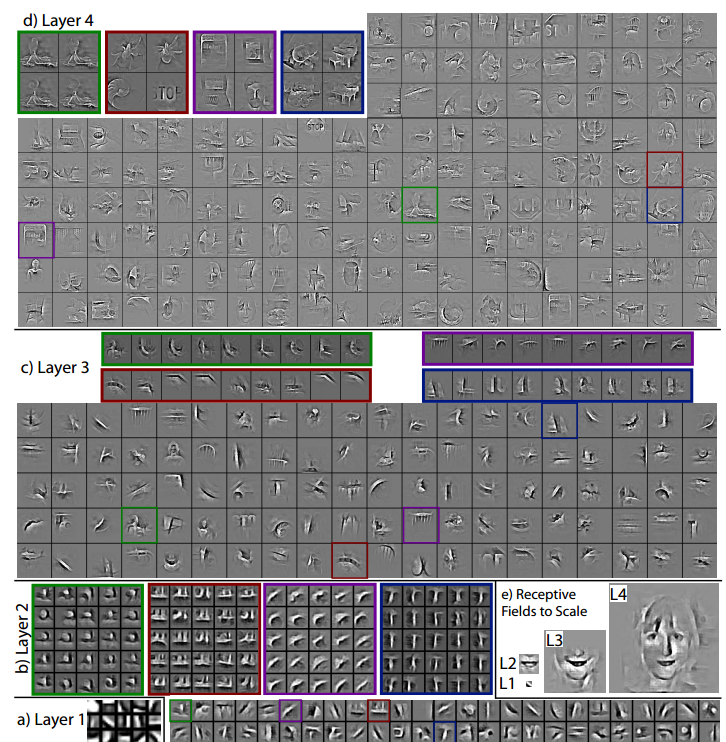
\includegraphics[scale=.5, angle=0]{Files/cnn-visualize.png}
    \caption[CNN Filters Visualizations]{CNN Filters Visualization \cite{zeiler2011adaptive}}
    \label{fig:visualize-cnn}
\end{figure}

\par

One of the important area in an unsupervised learning is generative models.  In next subsections we explain different aspects of generative models and how this work has made contribution in generative adversarial networks.

\section{Importance of Generative Models}

Generative model play crucial role in various field of artificial intelligence as they are capable of extracting high level latent representation of the data. Generative model tries to understand the data by learning their probability distribution over high-dimensional space. Generative model can helps in various field such as reinforcement learning. In reinforcement learning it can generate future state by learning the conditional distribution of the future states based on the current state and possible action that can be taken. In this ways we can take a possible action on current state by querying the model \cite{finn}. Generative models can also help in learning over mutli modal data. In multi modal data we have multiple correct output for an input. For instance images with captions and tags, videos contain visual and audio signals are type of multi modal data. Multi modal data are we hard to train on standard machine learning algorithms but generative models have proven that they can handle these type of data \cite{srivastava2012}. As this work focuses on synthetic/fake image generation, we briefly introduce and define it in next section.

%import the Image generative models have been used %for a wide variety of problems such as applying %various fancy filters to images, compression and %decompression of images, super resolution %\cite{1609.04802} and image inpainting %\cite{1607.07539}.
% One of the major advantages for image generation is %the easy availability and accessibility  of image %repositories \cite{celeba} , so it does not require %labeled dataset.





\section{Synthetic Image Generation}
Image generation is one the central research areas under the category of unsupervised learning. To understand unsupervised learning, lets consider supervised learning first. In supervised learning, when given data and its label we try to model a function that learns the mapping of data to its label. As complexity of the data grows, it becomes very hard to find a function that can cover all the features of the data. Deep learning takes advantage of this with higher-level learned
features defined in terms of lower-level features \cite{bengio2012deep}. In other words, we are trying to find the posterior probability distribution of an object in an image, $P(y|x)$.
In unsupervised learning, we are given the data sample but we don't have the target or the output label and so the model tries understand and model the whole data. There are several unsupervised machine learning algorithms such as KNN, clustering etc. Hence, image generation problem falls under the category of unsupervised learning, as we are trying to mimic the distribution of images present in the dataset over high dimensional space. In this work, we have synthesised the images of faces and digits based on  given conditions  such facial attributes which includes bald, type of hair, style of hairs, type of digit. Most widely used method before Generative Adversarial Network involved using probabilistic generative models, which are discussed in section 2.1. This work uses Generative Adversarial Network framework for image generation which was first introduced by Goodfellow \textit{et al.} \cite{Original-GAN}. But the proposed  framework was highly unstable and generated low quality images. 

\section{Motivation}


CNNs have shown excellent capability in classification task \cite{CNN-Better} but they require large amounts of labeled data. Labeling and gathering large dataset require a lot of human effort and money. For instance in case of egocentric images, it becomes very tedious and time consuming in labeling all the images. This work tries to reduce this by developing generative models which are capable of generating labeled data.
There has been lot of research  in the area of generative framework. After the first paper there have been lot of papers which have modified and tweaked the framework to produce quality data sample. There are various frameworks which have tried various approaches to make GAN work. 


\section{Objective}

In this work, we investigate various generative adversarial networks. And later apply it over a celeba \cite{celeba} and MNIST \cite{MNIST} dataset to produce a fake images which are conditioned on some specific attributes. This work aims at combining various best practises gathered from different research papers to create a stabilized generative adversarial network.  


\section{Organization}

To explain this work, we start with  \autoref{chap:RelatedWork}. In this chapter we look at various work done in the field of generative model and also examine different models based on generative adversarial network. In \autoref{chap:CNN}, we review the key building block of this work, which is the perceptron and later the convolutional neural network. Then in next \autoref{chap:GAN} we explain the concept of generative adversarial framework before discussing the modification done as part of this work in \autoref{chap:EGAN}. Later in \autoref{chap:EnR}, we present the experiments and results obtained when the framework shown in \autoref{chap:EGAN} is implemented.